\chapter{Interval Graphs}

In this chapter an overview of the MUIG and UUIG families will be given, with their characterization.

\todo[inline]{in the case of UUIG I want to find a more exhaustive characterization using MUUIG's families to use them in TSG. In this case it will be easy to proof complexity on TSG recognition}

\section{Mixed Unit Interval Graphs}
\label{sec:muig}

\todo[inline]{Show and describe every family with demos from Joos' article}

\subsection{Families}

Here we are going to define every family of forbidden induced subgraphs for MUUIG.

An important family of forbidden induced subgraphs in paper TSG: $\mathcal{R}_k$
\todo{improve introduction to this subsection}

\begin{figure}
\begin{center}
  \begin{scaletikzpicturetowidth}{\textwidth}
  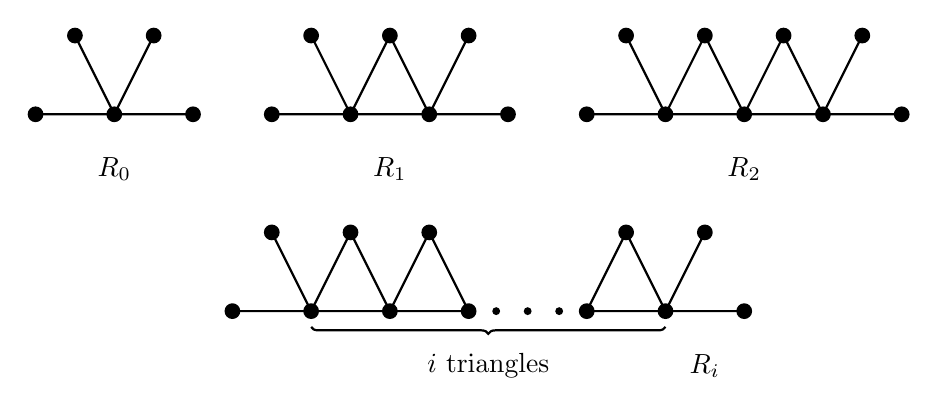
\begin{tikzpicture}[scale=1]
\def\ver{0.1} %size of a vertex
\def\x{1}

\def\xa{0.5}
\def\ya{0}

\def\xb{4}
\def\yb{0}

\def\xc{8}
\def\yc{0}

\def\xd{3.5}
\def\yd{-2.5}


%graph R_0
\path[fill] (\xa+0.5,\ya) circle (\ver);
\path[fill] (\xa+1,\ya+1) circle (\ver);
\path[fill] (\xa+2,\ya+1) circle (\ver);
\path[fill] (\xa+2.5,\ya) circle (\ver);
\path[fill] (\xa+1.5,\ya) circle (\ver);

\draw[thick] (\xa+0.5,\ya)--(\xa+1.5,\ya)--(\xa+1,\ya+1)
(\xa+2,\ya+1)--(\xa+1.5,\ya)--(\xa+2.5,\ya);

\node (1) at (\xa+1.5,\ya-0.7) {$R_0$};

%graph R_1
\path[fill] (\xb,\yb) circle (\ver);
\path[fill] (\xb+1,\yb) circle (\ver);
\path[fill] (\xb+2,\yb) circle (\ver);
\path[fill] (\xb+3,\yb) circle (\ver);
\path[fill] (\xb+0.5,\yb+1) circle (\ver);
\path[fill] (\xb+1.5,\yb+1) circle (\ver);
\path[fill] (\xb+2.5,\yb+1) circle (\ver);

\draw[thick] (\xb,\yb)--(\xb+1,\yb)--(\xb+2,\yb)--(\xb+3,\yb)
(\xb+0.5,\yb+1)--(\xb+1,\yb)--(\xb+1.5,\yb+1)--(\xb+2,\yb)--(\xb+2.5,\yb+1);

\node (1) at (\xb+1.5,\yb-0.7) {$R_1$};


%graph R_2
\path[fill] (\xc,\yc) circle (\ver);
\path[fill] (\xc+1,\yc) circle (\ver);
\path[fill] (\xc+2,\yc) circle (\ver);
\path[fill] (\xc+3,\yc) circle (\ver);
\path[fill] (\xc+4,\yc) circle (\ver);
\path[fill] (\xc+0.5,\yc+1) circle (\ver);
\path[fill] (\xc+1.5,\yc+1) circle (\ver);
\path[fill] (\xc+2.5,\yc+1) circle (\ver);
\path[fill] (\xc+3.5,\yc+1) circle (\ver);

\draw[thick] (\xc,\yc)--(\xc+1,\yc)--(\xc+2,\yc)--(\xc+3,\yc)--(\xc+4,\yc)
(\xc+0.5,\yc+1)--(\xc+1,\yc)--(\xc+1.5,\yc+1)--(\xc+2,\yc)--(\xc+2.5,\yc+1)--(\xc+3,\yc)--(\xc+3.5,\yc+1);

\node (1) at (\xc+2,\yc-0.7) {$R_2$};

%graph R_i
\path[fill] (\xd,\yd) circle (\ver);
\path[fill] (\xd+1,\yd) circle (\ver);
\path[fill] (\xd+2,\yd) circle (\ver);
\path[fill] (\xd+3,\yd) circle (\ver);
\path[fill] (\xd+4.5,\yd) circle (\ver);
\path[fill] (\xd+5.5,\yd) circle (\ver);
\path[fill] (\xd+6.5,\yd) circle (\ver);
\path[fill] (\xd+0.5,\yd+1) circle (\ver);
\path[fill] (\xd+1.5,\yd+1) circle (\ver);
\path[fill] (\xd+2.5,\yd+1) circle (\ver);
\path[fill] (\xd+5,\yd+1) circle (\ver);
\path[fill] (\xd+6,\yd+1) circle (\ver);

\fill (\xd+3.35,\yd) circle (\ver/2);
\fill (\xd+3.75,\yd) circle (\ver/2);
\fill (\xd+4.15,\yd) circle (\ver/2);

\draw[thick] (\xd,\yd)--(\xd+3,\yd)
(\xd+4.5,\yd)--(\xd+6.5,\yd)
(\xd+0.5,\yd+1)--(\xd+1,\yd)--(\xd+1.5,\yd+1)--(\xd+2,\yd)--(\xd+2.5,\yd+1)--(\xd+3,\yd)
(\xd+4.5,\yd)--(\xd+5,\yd+1)--(\xd+5.5,\yd)--(\xd+6,\yd+1);

\draw[thick,decoration={brace,mirror,raise=0.2cm},decorate] (\xd+1,\yd) -- (\xd+5.5,\yd)
node [pos=0.5,anchor=north,yshift=-0.4cm] {$i$ triangles};

\node (1) at (\xd+6,\yd-0.7) {$R_i$};

\end{tikzpicture}
\end{scaletikzpicturetowidth}
\end{center}
\caption{The class $\mathcal{R}$.}\label{graphsR}
\end{figure}


\lemma{$\mathcal{R}$ is a family of co-comparability graphs.}
\proof{If we recall Theorem \ref{theo:spanning}, in order to prove that $\mathcal{R}$ is a family of co-comparability graphs we will have to find a spanning order for every $R_i$ with $i \geq 0$. We will proceed to label our vertices with a mapping function $f: V \to \mathbb{N}$ such that $f(v) \in [1,|V|]$. This mapping will give us a spanning order by induction:

\begin{itemize}
  \item $i = 0$: We assign the number $1$ to the vertex with maximum degree $v_1$. We assign then the rest of the numbers to the other vertices. We see then that $\forall u < v < w : uw\in E \to uv \in E$ because every vertex is adjacent to $v_1$.

  \item $i = i+1$: We define $\lambda_i = 5+2i$ where $\lambda_i = |V(R_i)|$ (the size of the graph). We have two on each graph, where their labels are $\lambda_i+1$ and $\lambda_i+2$ and there are three new edges: $v_{\lambda_i}v_{\lambda_i-1},v_{\lambda_i}v_{\lambda_i+1},v_{\lambda_i}v_{\lambda_i+2} \in E$.

  By induction we only have to see if the new edges break our order. We can say that $v_{\lambda_i}v_{\lambda_i-1}$ and $v_{\lambda_i}v_{\lambda_i+1}$ do not break it because:

  $$\nexists k \in \mathbb{N} : i < k < i+1$$

  Finally, we see that $v_{\lambda_i}v_{\lambda_i+2}$ is a valid edge because $v_{\lambda_i}v_{\lambda_i+1}\in E$. \qed
\end{itemize}
}

\section{Unfettered Unit Interval Graphs}

\todo[inline]{Try to characterize with known forbidden families of subgraphs (from MUIG? and TSG article)}
